\documentclass[crop,tikz]{standalone}
\usepackage{tikz}
\usetikzlibrary{matrix,backgrounds,arrows.meta,fit,positioning,decorations.pathreplacing}
\begin{document}

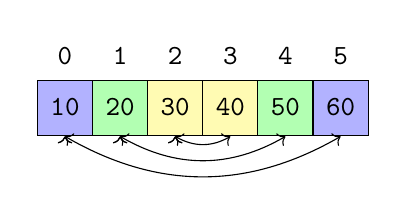
\begin{tikzpicture}[font=\ttfamily,
  array/.style={matrix of nodes,nodes={draw, fill=green!30,minimum size=7mm},column sep=-\pgflinewidth, row sep=0.5mm, nodes in empty cells,text height=1.5ex, text depth=.25ex,
    row 1/.style={nodes={draw=none, fill=none, minimum size=5mm}},
    row 2 column 1/.style={nodes={fill=blue!30}},
    row 2 column 6/.style={nodes={fill=blue!30}},
    row 2 column 2/.style={nodes={fill=green!30}},
    row 2 column 5/.style={nodes={fill=green!30}},
    row 2 column 3/.style={nodes={fill=yellow!30}},
    row 2 column 4/.style={nodes={fill=yellow!30}},
}]

\matrix[array] (array) {
 0 & 1 & 2 & 3 & 4 & 5 \\
  10 & 20 & 30 & 40 & 50 & 60 \\ };

\draw[<->] (array-2-1.south) edge[bend right] (array-2-6.south);
\draw[<->] (array-2-2.south) edge[bend right] (array-2-5.south);
\draw[<->] (array-2-3.south) edge[bend right] (array-2-4.south);

\end{tikzpicture}
\end{document}
